\documentclass{beamer}

\usepackage{mathtools}
\usetheme{Boadilla}
\usepackage{minted}
\usepackage{tikz}
\usepackage{amsmath}
\usepackage{physics}
\usetikzlibrary{decorations.markings}



%Information to be included in the title page:
\title{Path integral Monte Carlo: Lattice QCD}
\author{Damiano Scevola, Federico Tonetto}

\date{October 2024}

\begin{document}

\frame{\titlepage}

\begin{frame}{Path Integral Approach to Quantum Mechanics}
    Our goal is to compute quantum mechanical observables using the path integral approach. The central quantity we aim to compute is the correlation function:
    \begin{equation*}
        \langle x(t_2)x(t_1)\rangle = G(t) = \frac{\int Dx(t) x(t_2) x(t_1) e^{-S[x]}}{\int Dx \, e^{-S[x]}},
    \end{equation*}
    which represents a weighted average over paths, where the weight is determined by the action $S[x]$.
    To do so, we discretize the path $t_j = t_0 + ja, \quad j=0,...,N$.
\end{frame}

\begin{frame}{Numerical calculation of the propagator}
    Before calculating the correlation function, we see another application of the path integral formalism: the computation of the propagator.
    To do so, it is possible to shift the problem from quantum mechanics to numerical integration, indeed
    \begin{equation*}
        \bra{x}e^{-HT}\ket{x} \simeq A\int_0^{aN} dx_1...dx_{N-1} e^{-S_{lat} [x]},
    \end{equation*}
    hence, by computing the path integral on the left side, it is possible to compute the propagator given the ground state and the ground state energy. We have than it numerically by using the Vegas library.  We observe that, in dimension greater than 1, this procedure is not efficient.
\end{frame}

\begin{frame}{Harmonic oscillator}
    We have computed the propagator for the harmonic oscillator.
    \begin{figure}
        \centering
        \includegraphics[width=0.5\linewidth]{harmonic_oscillator_numerical_propagator.png}
        \caption{Propagators value of the harmonic oscillator versus time.}
        \label{fig:harmonic}
    \end{figure}
\end{frame}

\begin{frame}{Anharmonic oscillator}
    We have also done it for the anharmonic oscillator $V(x) = \frac{x^4}{4}$
    \begin{figure}
        \centering
        \includegraphics[width=0.5\linewidth]{anharmonic_oscillator_numerical.png}
        \caption{Propagators value of the anharmonic oscillator versus time. We observe that the values are shifted due to renormalization effects.}
        \label{fig:enter-label}
    \end{figure}
\end{frame}
% Slide 2: Monte Carlo Approach Explanation
\begin{frame}{Monte Carlo Approach}
    A more convenient way to compute path integrals is to generate a large number of configurations at each time step:
    \[
    x(n) = (x_1, \dots, x_{N_{cf}}), \quad n = a, 2a, \dots, Na, \text{ with } T = Na,
    \]
    where the configurations follow the probability distribution determined by $e^{-S[x]}$. For this, we use the Metropolis algorithm.
\end{frame}

% Slide 3: Metropolis Algorithm Code
\begin{frame}[fragile]{Metropolis Algorithm}
        \begin{minted}{python}
def update_path(path, S_per_timeslice, eps: np.float64):
    N = path.shape[0]
    for j in range(N):
        # Save the original value
        old_x = path[j]
        old_Sj = S_per_timeslice(j, path)
        # Propose a new value for path[j]
        path[j] += np.random.uniform(-eps, eps)
        # Calculate the change in action
        dS = S_per_timeslice(j, path) - old_Sj
        # Accept or reject the new value based on Metropolis criterion
        if dS > 0 and np.exp(-dS) < np.random.uniform(0, 1):
            # Restore old value if not accepted
            path[j] = old_x
    \end{minted}
    This algorithm ensures that paths with lower action are favored while allowing for random fluctuations.
\end{frame}

% Slide 4: Monte Carlo Process Explanation
\begin{frame}{Monte Carlo Process Overview}
    In general, we perform the following steps:
    \begin{itemize}
        \item Thermalize the lattice by updating all the paths for a given number of steps ($\approx 5 \times N_{cor}$).
        \item Update the path $N_{cor}$ times, then compute a functional of interest. Repeat this process $N \times N_{cf}$ times.
        \item Store the results in a matrix.
        \item Finally, compute averages and errors from the matrix.
    \end{itemize}
\end{frame}

    % Slide 5: Bootstrap Procedure
\begin{frame}[fragile]
    \frametitle{Improvements: Bootstrap Procedure}
    \begin{minted}{python}
for i in range(N_copies):
    s = np.zeros((N_cf, N), dtype=np.float64)
    for row in range(N_cf):
        i = np.int32(np.random.uniform(0, N_cf))
        for n in range(N):
            s[row][n] = functional_samples[i][n]
    for n in range(N):
        avgs[i, n] = np.sum(s[:, n]) / N_cf
        stds[i, n] = np.sum((s[:, n] - avgs[i, n]) ** 2)
                    / (N_cf * np.sqrt(N_cf))
return avgs, stds
    \end{minted}
\end{frame}

% Slide 6: Binning Method
\begin{frame}{Binning Method}
    The binning procedure is useful when $N_{cf}$ is large and $N_{cor}$ is low. Instead of storing all $N_{cf}$ values, we store only a subset. To achieve this, we define a bin size, $bin_{size}$, and store only the average of the points within each bin.
\end{frame}

% Slide 7: Applications Overview
\begin{frame}{Applications}
    We have computed the difference between the first excited state and the ground state using the formula:
    \begin{equation*}
        \Delta E_n = \log \left| \frac{G_n}{G_{n+1}} \right|
    \end{equation*}
    for both the harmonic oscillator and the anharmonic oscillator (where $V = \frac{x^4}{4}$). Additionally, we computed the cubic correlator:
    \begin{equation*}
        \langle x^3(t_1)x^3(t_2) \rangle
    \end{equation*}
    for the harmonic oscillator.
\end{frame}

% Slide 8: Harmonic Oscillator Results
\begin{frame}{Results for the Harmonic Oscillator}
    \begin{figure}
        \centering
        \includegraphics[width=0.5\linewidth]{harmonic_oscillator.png}
        \caption{Monte Carlo values $\Delta E(t) = \log \left( \frac{G_n}{G_{n+1}} \right)$ plotted versus $t$ for the harmonic oscillator. The exact result, $\Delta E = \frac{1}{2}$, is shown with a line.}
        \label{fig:harmonic_oscillator_basic}
    \end{figure}
\end{frame}

% Slide 9: Anharmonic Oscillator Results
\begin{frame}{Results for the Anharmonic Oscillator}
    \begin{figure}
        \centering
        \includegraphics[width=0.5\linewidth]{anharmonic_oscillator_basic.png}
        \caption{Monte Carlo values $\Delta E(t) = \log \left( \frac{G_n}{G_{n+1}} \right)$ for the anharmonic oscillator. The exact result, $\Delta E$, is shown with a line and is computed by solving the Schrödinger equation. Renormalization causes a shift.}
        \label{fig:anharmonic_oscillator_basic}
    \end{figure}
\end{frame}

% Slide 10: Cubic correlator Results
\begin{frame}{Cubic correlator}
    \begin{figure}
        \centering
        \includegraphics[width=0.5\linewidth]{cubic_propagator.png}
        \caption{Monte Carlo values of $\Delta E(t) = \log \left( \frac{G_n}{G_{n+1}} \right)$ for the harmonic oscillator. The exact value is reached from above when the source and sink are the same.}
        \label{fig:cubic_propagator}
    \end{figure}
\end{frame}

% Slide 11: Comment on Thermalization and Binning
\begin{frame}{A Comment on Thermalization and Binning}
    If $N_{cor}$ is too small, the values become statistically correlated, leading to unreliable error estimates. This issue can be mitigated by increasing the bin size.

    \begin{figure}[ht]
    \begin{minipage}[b]{0.4\linewidth}
        \centering
        \includegraphics[width=\textwidth]{harmonic_oscillator_with_low_thermalization.png}
        \caption{Monte Carlo values $\Delta E(t)$ for the harmonic oscillator with $N_{cor}=1$. The error bars are unreliable.}
        \label{fig:harmonic_oscillator_with_low_thermalization}
    \end{minipage}
    \hspace{0.5cm}
    \begin{minipage}[b]{0.4\linewidth}
        \centering
        \includegraphics[width=\textwidth]{harmonic_oscillator_with_low_thermalization_and_binning.png}
        \caption{Monte Carlo values $\Delta E(t)$ with $N_{cor}=1$ and $bin_{size}=20$. The error bars looks like before.}
        \label{fig:harmonic_oscillator_with_low_thermalization_and_binning}
    \end{minipage}
    \end{figure}
\end{frame}

% Slide 12: Lattice Approximation of Derivatives
\begin{frame}{Derivative in Lattice Approximation}
    On the lattice, derivatives are replaced by differences. We use the following approximation:
    \begin{align*}
        \frac{\partial^2 \phi}{\partial x^2} = \Delta_x^{(2)} \phi - \frac{a^2}{12} \left( \Delta_x^{(2)} \right)^2 \phi + O(a^4),
    \end{align*}
    where
    \begin{equation*}
        \Delta_x^{(2)} = \frac{\phi(x+a) - 2\phi(x) + \phi(x-a)}{a^2}.
    \end{equation*}
\end{frame}

% Slide 13: Harmonic Oscillator with Improved Action
\begin{frame}{Harmonic oscillator with improved action}
    To make use of the previous formula, it is possible to integrate by parts inside the action and, after the discretization, obtain the following action
    \begin{equation*}
            S_{imp}[x] = \sum_{j=0}^{N-1} a  \left[-\frac{1}{2}x_j \left(\Delta^{(2)} -a^2 \frac{(\Delta^{(2)})^2}{12} -1 \right)x_j \right].
    \end{equation*}
    We compute again $\Delta E$ but now we update the path with the new action.
\end{frame}


% Slide: Numerical Ghosts
\begin{frame}{Numerical Ghosts}
    By solving the equation of motion for the harmonic oscillator, it is possible to find two different frequency solutions. The first corresponds to an improvement over the non-improved action, while the second is a so-called "numerical ghost". This ghost introduces an additional state that shifts the values of $\Delta E$, causing the energies to rise from below.
\end{frame}

% Slide: Change of Coordinates
\begin{frame}{Change of Coordinates}
    To eliminate the numerical ghosts, we can use a transformation that removes the extra states. This is done through an infinitesimal coordinate transformation, which effectively shifts the potential. After applying this transformation, the action becomes:
    \begin{equation*}
        S_{\text{imp}}[x] = \sum_{j=0}^{N-1} a  \left[-\frac{1}{2}x_j \Delta^{(2)} x_j + V_{\text{imp}}(x_j) \right],
    \end{equation*}
    where the improved potential is given by:
    \begin{equation*}
        V_{\text{imp}}(x_j) = \frac{1}{2}x_j^2 \left(1+\frac{a^2}{12}\right) + O(a^4).
    \end{equation*}
\end{frame}

% Slide: Results (Harmonic Oscillator)
\begin{frame}{Results for the Harmonic Oscillator}
    \begin{figure}[ht]
        \begin{minipage}[b]{0.4\linewidth}
            \centering
            \includegraphics[width=\textwidth]{Harmonic_oscillator_with_improved_action.png}
            \caption{Monte Carlo values of $\Delta E(t) = \log\left( \frac{G_n}{G_{n+1}} \right)$ plotted versus $t$ for the harmonic oscillator using the improved action. A numerical ghost with negative norm is observed.}
            \label{fig:Harmonic_oscillator_with_improved_action}
        \end{minipage}
        \hspace{0.5cm}
        \begin{minipage}[b]{0.4\linewidth}
            \centering
            \includegraphics[width=\textwidth]{harmonic_oscillator_with_no_ghosts.png}
            \caption{Monte Carlo values $\Delta E(t) = \log\left( \frac{G_n}{G_{n+1}} \right)$ plotted versus $t$ for the harmonic oscillator using the improved potential. There are not states with negative norm.}
            \label{fig:harmonic_oscillator_with_no_ghosts}
        \end{minipage}
    \end{figure}
\end{frame}

% Slide: Ghosts for Anharmonic Oscillator
\begin{frame}{Ghosts in the Anharmonic Oscillator}
    We also considered the case of the anharmonic oscillator, where the potential is given by:
    \begin{equation*}
        V(x) = \frac{1}{2}x^2(1+2x^2).
    \end{equation*}
    Even in this case, a change of coordinates can be applied to remove the ghosts. With this transformation, the improved potential becomes:
    \begin{equation*}
        V_{\text{imp}}(x) = \frac{1}{2}x^2(1+2x^2) + \frac{a^2}{24} \left(x + 4x^3\right)^2 - \frac{ax^2}{2} + \frac{a^3x^4}{8}.
    \end{equation*}
\end{frame}

% Slide: Results (Anharmonic Oscillator)
\begin{frame}{Results for the Anharmonic Oscillator}
    \begin{figure}[ht]
        \begin{minipage}[b]{0.4\linewidth}
            \centering
            \includegraphics[width=\textwidth]{anharmonic_oscillator_with_improved_action.png}
            \caption{Monte Carlo values of $\Delta E(t) = \log\left( \frac{G_n}{G_{n+1}} \right)$ plotted versus $t$ for the anharmonic oscillator using the improved action. A ghost with negative norm is observed.}
            \label{fig:anharmonic_oscillator_with_improved_action}
        \end{minipage}
        \hspace{0.5cm}
        \begin{minipage}[b]{0.4\linewidth}
            \centering
            \includegraphics[width=\textwidth]{anharmonic_oscillator_with_no_ghosts.png}
            \caption{Monte Carlo values of $ \Delta E(t)= \log\left( \frac{G_n}{G_{n+1}} \right)$ plotted versus $t$ for the anharmonic oscillator using the improved potential. There are not states with negative norm.}
            \label{fig:anharmonic_oscillator_with_no_ghosts}
        \end{minipage}
    \end{figure}
\end{frame}

% Slide: Renormalization Effects
\begin{frame}{Renormalization Effects}
    As is typical with non-free potentials, there are renormalization effects to consider. In the case of the anharmonic oscillator, the change of coordinates does not account for these effects, which can introduce errors of order $\mathcal{O}(a)$.
\end{frame}

\begin{frame}{Calculation of the renormalization effects}
    To compute the renormalization effects we have calculated the exact $\Delta E$  by solving the Schroedinger equation. Then we have computed the difference between the exact $\Delta E$  and the average of the first 5 points of the path integral. We have done this both for $a=\frac{1}{2}$ and $a= \frac{1}{4}$.
    We have obtained
    \begin{align*}
        a &= 0.5 \Rightarrow \delta = 0.11 \\
        a &= 0.25 \Rightarrow \delta = 0.04.
    \end{align*}
\end{frame}

\begin{frame}{Calculation of the correction factor}
    By adjusting the coefficient of $x^2$ in the potential it is possible to reduce this effect. Let $z$ be that coefficient.
    We know that there exists a value of $z$ that eliminates the discrepancy.
    Hence we have created a function that, given an interval, computes the smallest sub interval in which the theorem of the zeros still holds. We have parallelized the process by dividing the interval in a given numbers of slices.
\end{frame}

\begin{frame}{Result}
    We have obtained the following value
    \begin{equation*}
        z = 1.02 \pm 0.31.
    \end{equation*}
    With this value $\Delta E$ becomes
    \begin{figure}
        \centering
        \includegraphics[width=0.5\linewidth]{anharmonic_oscillator_with_correct_z.png}
        \caption{Monte Carlo values of $\Delta E(t) = \log\left( \frac{G_n}{G_{n+1}} \right)$ plotted versus $t$ for the anharmonic oscillator using the correct value of $z$.}
        \label{fig:anharmonic_oscillator_with_correct_z}
    \end{figure}
\end{frame}


\begin{frame}
    \begingroup
      \centering
      \begin{beamercolorbox}[sep=12pt,center,colsep=-4bp,rounded=true,shadow=true]{section title}
        \usebeamerfont{section title}Lattice QCD\par
      \end{beamercolorbox}
    \endgroup
  \end{frame}



\begin{frame}{Field discretization}
    Discretize spacetime: $N$ points per spacetime direction
    \begin{figure}
        \centering
        \includegraphics[width=0.5\linewidth]{lattice.png}
        \caption{Lattice discretization for $d=2$, $N=4$}
        \label{fig:lattice}
    \end{figure}
\end{frame}


\begin{frame}[fragile]
    \frametitle{Field configuration encoding}
    \begin{itemize}
        \item Each link is an $SU(3)$ matrix

        \item There is a link for each spacetime direction, for each spacetime point ($d \cdot N^d$ links in total).

        \item Use a complex \texttt{numpy} array with shape $(N^d, d, 3, 3)$.

        \item Nodes indexed by integers $i \in \{0,\ldots,N^d-1\}$

        \item Spacetime coordinates: ordered array (length $d$) of digits given by the base-$N$ conversion of the index $i$.

        \item Periodic boundary conditions
    \end{itemize}
\end{frame}

\begin{frame}[fragile]
    \frametitle{Paths and loops}
    Wilson loops:
    \begin{equation*}
        W(\mathcal{C}) = \frac{1}{3} Re\ tr (\mathcal{C})
    \end{equation*}
    $\mathcal{C}$: product of links


    \begin{minted}{python}
    compute_path(links, [1,0], [+1,+2,+1,+2,-1,-1,-2,-2])
    \end{minted}

    \begin{figure}
        \centering
        \includegraphics[width=0.3\linewidth]{wilsonloop.png}
        \caption{Example of a Wilson loop in a 4 x 4 2d lattice. $\mu \leftrightarrow 1$, $\nu \leftrightarrow 2$ }
        \label{fig:wilson-loop}
    \end{figure}

\end{frame}

\begin{frame}
    \frametitle{Plaquettes and Wilson action}
    Wilson action:
    \begin{equation*}
        S_{Wil} = \beta \sum_{x, \mu > \nu} (1-P_{\mu\nu}(x))
    \end{equation*}

    where $P_{\mu\nu}(x)$ is the plaquette operator.

    \begin{figure}
        \centering

        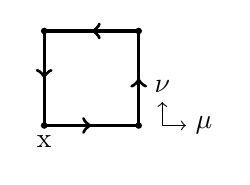
\begin{tikzpicture}[scale=0.6]

            \draw[->] (2.5, 0) -- (2.5, 0.5) node[above] {$\nu$};
            \draw[->] (2.5, 0) -- (3, 0) node[right] {$\mu$};

            \begin{scope}[very thick,decoration={
                markings,
                mark=at position 0.5 with {\arrow{>}}}
                ]
                \draw[postaction={decorate}] (0,0)--(2,0);
                \draw[postaction={decorate}] (2,0)--(2,2);
                \draw[postaction={decorate}] (2,2)--(0,2);
                \draw[postaction={decorate}] (0,2)--(0,0);
            \end{scope}

            \draw (0,0) node[below] {x};


            \fill (0,0) circle (2pt);
            \fill (0,2) circle (2pt);
            \fill (2,0) circle (2pt);
            \fill (2,2) circle (2pt);

            \end{tikzpicture}

        \caption{Plaquette operator $P_{\mu\nu}(x)$}
        \label{fig:enter-label}
    \end{figure}

    \begin{itemize}
        \item This is the most local, gauge invariant action that one can build.
        \item Poincarè symmetry is discretized.
        \item This action is the correct one in the limit $a \rightarrow 0$
        \item Discretization error of order $\mathcal{O}(a^2)$
    \end{itemize}






\end{frame}

\begin{frame}
    \frametitle{Metropolis update for Wilson action}
    \begin{itemize}
        \item Update $U_{\mu}(x)$ \texttt{hits=10} times
        \item Updating once means $U_{\mu}(x) \rightarrow MU_{\mu}(x)$ where $M \in SU(3)$ is a random SU(3) matrix s.t. $|M - \mathbb{I}_{3}| \sim \epsilon \ll 1$
        \item Check metropolis acceptance condition each hit
        \item $\Delta S = S[MU_{\mu}(x) - U_{\mu}(x)]$
        \item Factorize $U_{\mu}(x)$ and compute $\Gamma_{\mu}(x)$ before \texttt{hits} to save time.
    \end{itemize}

    \begin{figure}
        \centering
        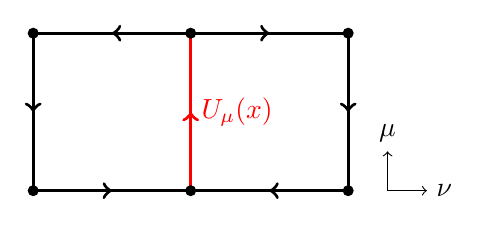
\begin{tikzpicture}

            \draw[->] (4.5, 0) -- (4.5, 0.5) node[above] {$\mu$};
            \draw[->] (4.5, 0) -- (5, 0) node[right] {$\nu$};

            \begin{scope}[very thick,decoration={
                markings,
                mark=at position 0.5 with {\arrow{>}}}
                ]
                \draw[postaction={decorate}] (2,2)--(0,2);
                \draw[postaction={decorate}] (0,2)--(0,0);
                \draw[postaction={decorate}] (0,0)--(2,0);

                \draw[postaction={decorate}] (2,2)--(4,2);
                \draw[postaction={decorate}] (4,2)--(4,0);
                \draw[postaction={decorate}] (4,0)--(2,0);

                \draw[red, postaction={decorate}] (2,0) -- (2,2) node[midway, right] {$U_{\mu}(x)$};
            \end{scope}


            \fill (0,0) circle (2pt);
            \fill (4,0) circle (2pt);
            \fill (4,2) circle (2pt);
            \fill (0,2) circle (2pt);
            \fill (2,0) circle (2pt);
            \fill (2,2) circle (2pt);

            \end{tikzpicture}
            \caption{Plaquettes contributing to the action in each spacetime direction.}
        \label{fig:enter-label}
    \end{figure}

\end{frame}

\begin{frame}
    \frametitle{Rectangles and improved action}
    Improved action gives $\mathcal{O}(a^4)$ error (instead of $\mathcal{O}(a^2)$).

    \begin{equation*}
        S = -\beta \sum_{x, \mu > \nu} \left[\frac{5}{3} \frac{P_{\mu\nu}(x)}{u_0^4} - \frac{R_{\mu\nu}(x) + R_{\nu\mu}(x)}{12 u_0^6}\right]
    \end{equation*}

    $R_{\mu\nu}(x)$ is the rectangle operator

    $u_0 \in \mathbb{R}$ accounts for tadpole improvement

    \begin{figure}
        \centering
        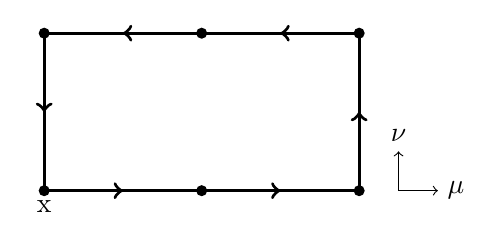
\begin{tikzpicture}

            \draw[->] (4.5, 0) -- (4.5, 0.5) node[above] {$\nu$};
            \draw[->] (4.5, 0) -- (5, 0) node[right] {$\mu$};

            \begin{scope}[very thick,decoration={
                markings,
                mark=at position 0.5 with {\arrow{>}}}
                ]
                \draw[postaction={decorate}] (0,0)--(2,0);
                \draw[postaction={decorate}] (2,0)--(4,0);
                \draw[postaction={decorate}] (4,0)--(4,2);

                \draw[postaction={decorate}] (4,2)--(2,2);
                \draw[postaction={decorate}] (2,2)--(0,2);
                \draw[postaction={decorate}] (0,2)--(0,0);
            \end{scope}


            \fill (0,0) circle (2pt);
            \fill (4,0) circle (2pt);
            \fill (4,2) circle (2pt);
            \fill (0,2) circle (2pt);
            \fill (2,0) circle (2pt);
            \fill (2,2) circle (2pt);

            \draw (0,0) node[below] {x};

            \end{tikzpicture}
            \caption{Rectangle operator $R_{\mu\nu}(x)$}
        \label{fig:enter-label}
    \end{figure}

\end{frame}

\begin{frame}
    \frametitle{Metropolis update for improved action}
    Six rectangle contributions $\forall \nu$
    \begin{figure}
        \centering
        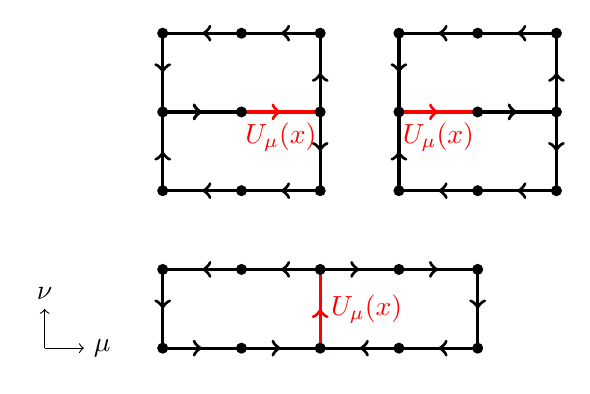
\begin{tikzpicture}

            \draw[->] (-4.5, 0) -- (-4.5, 0.5) node[above] {$\nu$};
            \draw[->] (-4.5, 0) -- (-4, 0) node[right] {$\mu$};

            \begin{scope}[very thick,decoration={
                markings,
                mark=at position 0.5 with {\arrow{>}}}
                ]
                \draw[postaction={decorate}] (-1,1)--(-2,1);
                \draw[postaction={decorate}] (-2,1)--(-3,1);
                \draw[postaction={decorate}] (-3,1)--(-3,0);
                \draw[postaction={decorate}] (-3,0)--(-2,0);
                \draw[postaction={decorate}] (-2,0)--(-1,0);

                \draw[postaction={decorate}] (-1,1)--(0,1);
                \draw[postaction={decorate}] (0,1)--(1,1);
                \draw[postaction={decorate}] (1,1)--(1,0);
                \draw[postaction={decorate}] (1,0)--(0,0);
                \draw[postaction={decorate}] (0,0)--(-1,0);

                \draw[red, postaction={decorate}] (-1,0) -- (-1,1) node[midway, right] {$U_{\mu}(x)$};





                \draw[postaction={decorate}] (-1,3)--(-1,4);
                \draw[postaction={decorate}] (-1,4)--(-2,4);
                \draw[postaction={decorate}] (-2,4)--(-3,4);
                \draw[postaction={decorate}] (-3,4)--(-3,3);
                \draw[postaction={decorate}] (-3,3)--(-2,3);
                \draw[postaction={decorate}] (-1,3)--(-1,2);
                \draw[postaction={decorate}] (-1,2)--(-2,2);
                \draw[postaction={decorate}] (-2,2)--(-3,2);
                \draw[postaction={decorate}] (-3,2)--(-3,3);
                \draw[postaction={decorate}] (-3,3)--(-2,3);
                \draw[red, postaction={decorate}] (-2,3) -- (-1,3) node[midway, below] {$U_{\mu}(x)$};


                \draw[postaction={decorate}] (2,3)--(2,4);
                \draw[postaction={decorate}] (2,4)--(1,4);
                \draw[postaction={decorate}] (1,4)--(0,4);
                \draw[postaction={decorate}] (0,4)--(0,3);
                \draw[postaction={decorate}] (1,3)--(2,3);
                \draw[postaction={decorate}] (2,3)--(2,2);
                \draw[postaction={decorate}] (2,2)--(1,2);
                \draw[postaction={decorate}] (1,2)--(0,2);
                \draw[postaction={decorate}] (0,2)--(0,3);
                \draw[postaction={decorate}] (1,3)--(2,3);
                \draw[red, postaction={decorate}] (0,3) -- (1,3) node[midway, below] {$U_{\mu}(x)$};


            \end{scope}


            \fill (-3,0) circle (2pt);
            \fill (-2,0) circle (2pt);
            \fill (-1,0) circle (2pt);
            \fill (0,0) circle (2pt);
            \fill (1,0) circle (2pt);
            \fill (-3,1) circle (2pt);
            \fill (-2,1) circle (2pt);
            \fill (-1,1) circle (2pt);
            \fill (0,1) circle (2pt);
            \fill (1,1) circle (2pt);

            \fill (-1,3) circle (2pt);
            \fill (-1,4) circle (2pt);
            \fill (-2,4) circle (2pt);
            \fill (-3,4) circle (2pt);
            \fill (-3,3) circle (2pt);
            \fill (-2,3) circle (2pt);
            \fill (-1,2) circle (2pt);
            \fill (-2,2) circle (2pt);
            \fill (-3,2) circle (2pt);

            \fill (2,3) circle (2pt);
            \fill (2,4) circle (2pt);
            \fill (1,4) circle (2pt);
            \fill (0,4) circle (2pt);
            \fill (0,3) circle (2pt);
            \fill (1,3) circle (2pt);
            \fill (2,2) circle (2pt);
            \fill (1,2) circle (2pt);
            \fill (0,2) circle (2pt);

            \end{tikzpicture}
            \caption{Rectangles contributing to the action in each spacetime direction where the link $U_{\mu}(x)$ appears.}
        \label{fig:enter-label}
    \end{figure}
\end{frame}

\begin{frame}
    \frametitle{Rotational invariance of the lattice}
    \begin{itemize}
        \item Lattice is symmetric under permutations of spacetime directions (i.e. rotations)
        \item We can draw more samples for each lattice update.
        \item \texttt{compute\_wilson\_loop\_average\_fixed\_frame(links, loops, rotated\_axes)} exploits only translational invariance
        \item\texttt{rotated\_axes} is a permutation of the first $d$ integers
        \item \texttt{generate\_wilson\_samples} calls \texttt{compute\_wilson\_loop\_average\_fixed\_frame} $d!$ times (or $(d-1)!$ times, see smearing) for each loop, for each sample.
    \end{itemize}

\end{frame}

\begin{frame}
    \frametitle{Initialization and thermalization}
    \begin{itemize}
        \item All lattice links are initialized to $\mathbb{I}_3$
        \item Perform \texttt{N\_cor * thermalization\_its} iterations of a full lattice update to thermalize
        \item After this, start drawing samples
    \end{itemize}
\end{frame}

\begin{frame}
    \frametitle{Computing Wilson loop averages}
    \begin{itemize}
        \item Prepare a list of loops in step notation (no symmetry-equivalent loops shall be included)
        \item For each rotational configuration, for each loop in the list, we call \texttt{compute\_wilson\_loop\_average\_fixed\_frame}
        \item Average results
        \item Repeat \texttt{N\_cf} times
        \item Apply bootstrap procedure for error estimation
    \end{itemize}
\end{frame}

\begin{frame}
    \frametitle{Example of $a \times a$ and $a \times 2a$ Wilson loops}
    With $N=8$ and $a=0.25 \  fm$ ($\beta=5.5$ for Wilson action, $\beta=1.719$ and $u_0=0.797$  for improved action), we computed the following two loops:
    \begin{figure}
        \centering
        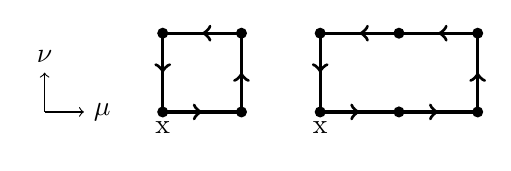
\begin{tikzpicture}

            \draw[->] (-1.5, 0) -- (-1.5, 0.5) node[above] {$\nu$};
            \draw[->] (-1.5, 0) -- (-1, 0) node[right] {$\mu$};

            \begin{scope}[very thick,decoration={
                markings,
                mark=at position 0.5 with {\arrow{>}}}
                ]
                \draw[postaction={decorate}] (0,0)--(1,0);
                \draw[postaction={decorate}] (1,0)--(1,1);
                \draw[postaction={decorate}] (1,1)--(0,1);
                \draw[postaction={decorate}] (0,1)--(0,0);

                \draw[postaction={decorate}] (2,0)--(3,0);
                \draw[postaction={decorate}] (3,0)--(4,0);
                \draw[postaction={decorate}] (4,0)--(4,1);
                \draw[postaction={decorate}] (4,1)--(3,1);
                \draw[postaction={decorate}] (3,1)--(2,1);
                \draw[postaction={decorate}] (2,1)--(2,0);
            \end{scope}


            \fill (0,0) circle (2pt);
            \fill (1,0) circle (2pt);
            \fill (1,1) circle (2pt);
            \fill (0,1) circle (2pt);
            \fill (2,0) circle (2pt);
            \fill (2,1) circle (2pt);
            \fill (3,0) circle (2pt);
            \fill (3,1) circle (2pt);
            \fill (4,0) circle (2pt);
            \fill (4,1) circle (2pt);

            \draw (0,0) node[below] {x};
            \draw (2,0) node[below] {x};

            \end{tikzpicture}
            \caption{Wilson loops $a \times a$ and $2a \times a$}
        \label{fig:enter-label}
    \end{figure}
    \begin{center}
    \begin{tabular}{||c | c c | c c||}
     \hline
     Loop & Wilson & Expected & Improved & Expected \\ [0.5ex]
     \hline\hline
     $a \times a$ & $0.498 \pm 0.001$ & $0.50$ & $0.5413 \pm 0.0005$ & $0.54$ \\
     \hline
     $2a \times a$ & $0.261 \pm 0.001$ & 0.26 & $0.2832 \pm 0.0006$ & 0.28 \\
     \hline
    \end{tabular}
    \end{center}

\end{frame}

\begin{frame}
    \frametitle{Static quark-antiquark potential}
    Potential between a quark $q$ and the corresponding antiquark $\bar{q}$ in the static $m_q \rightarrow \infty$ limit given by:
    \begin{equation*}
        W(r,t) \xrightarrow{t \rightarrow \infty} const\ e^{-V(r) t}
    \end{equation*}
    $W(r, t)$ is a Wilson loop like:
    \begin{figure}
        \centering
        \includegraphics[width=0.3\linewidth]{quark.png}
        \caption{Wilson loop for computing the potential.}
        \label{fig:enter-label}
    \end{figure}
    If we compute $W(r,t)$ and $W(r, t+a)$ with large $t$, we have:
    \begin{equation*}
        a \cdot V(r) = \log\left|\frac{W(r,t)}{W(r,t+a)}\right|
    \end{equation*}
\end{frame}

\begin{frame}
    \frametitle{Smearing}
    Numerical trick to hasten convergence: link smearing after first thermalization.
    \begin{itemize}
        \item Copy the current field configuration
        \item For each purely spacial link, apply smearing operator $(1+\epsilon a^2 \Delta^{(2)})$,
        \item $\Delta^{(2)}$ is the discretized gauge covariant derivative (use old links)
        \item Repeat $n$ times
    \end{itemize}
    Rotational symmetry broken between space and time.
\end{frame}

\begin{frame}
    \frametitle{Loops contributing to the first points of the potential}
    Spacial separations of the quark-antiquark pair up to $r=3$ (in units of $a$):
    \begin{center}
    \begin{tabular}{c c c }
     (0,0,1) & (0,1,1) & (1,1,1) \\
     (0,0,2) & (0,1,2) & (1,1,2) \\
     (0,2,2) & (1,2,2) & (0,0,3) \\
    \end{tabular}
    \end{center}
    These tuples are generated in non-decreasing order once, and then they are rotated in all the $6$ rotational configurations of the spacial directions.

    We will have $V(r)$ points for $r$ equals (in units of $a$):
    $$1, \sqrt{2}, \sqrt{3}, 2, \sqrt{5}, \sqrt{6}, \sqrt{8}, 3$$
    There will be two points for $r=3$.
\end{frame}

\begin{frame}
    \frametitle{Non-planar Wilson loops}
    Given a spacial separation $(x,y,z)$ between the two quarks loops are constructed as follows:
    \begin{itemize}
        \item start from the first quark in $(0,0,0)$
        \item do steps only in spacial directions to reach $(x,y,z)$
        \item do $t$ (or $t+a$) steps in the temporal direction
        \item do steps only in spacial directions to reach $(0,0,0)$
        \item do $t$ (or $t+a$) steps in the negative temporal direction
    \end{itemize}
    The spacial part of the loop can be arbitrairly complicated.
    However, the leading order contribution is given only by least-steps loops.

    If there is more than one non-zero coordinate, loops are non-planar.
\end{frame}

\begin{frame}
    \frametitle{Static quark-antiquark potential: results and fit}
    The parameters of our simulation:
    \begin{itemize}
        \item $N=8$ lattice points in each spacetime direction
        \item $a=0.25\ fm$
        \item $\beta = 5.5$ for Wilson action
        \item $\beta = 1.719$ and $u_0 = 0.797$ for improved action
        \item $\epsilon_{smear} = 1/12$
        \item $n_{smear} = 4$
        \item $N_{cor} = 50$
        \item $N_{cf} = 5$
        \item $N_{cor} = 50$
        \item $t = 2$ loop temporal width
    \end{itemize}
    Fit function:
    $$V(r) = ar - \frac{b}{r} + c$$
\end{frame}

\begin{frame}
\frametitle{Potential: Wilson action, no smearing}
\begin{figure}
    \centering
    \includegraphics[width=0.8\linewidth]{output1.png}
\end{figure}
\end{frame}

\begin{frame}
\frametitle{Potential: Wilson action, with smearing}
\begin{figure}
    \centering
    \includegraphics[width=0.8\linewidth]{output2.png}
\end{figure}
\end{frame}

\begin{frame}
\frametitle{Potential: improved action, no smearing}
\begin{figure}
    \centering
    \includegraphics[width=0.8\linewidth]{output3.png}
\end{figure}
\end{frame}

\begin{frame}
\frametitle{Potential: improved action, with smearing}
\begin{figure}
    \centering
    \includegraphics[width=0.8\linewidth]{output4.png}
\end{figure}
\end{frame}






\end{document}
